\documentclass{standalone}
\usepackage{pgfplots}
\pgfplotsset{compat=1.18}

\begin{document}
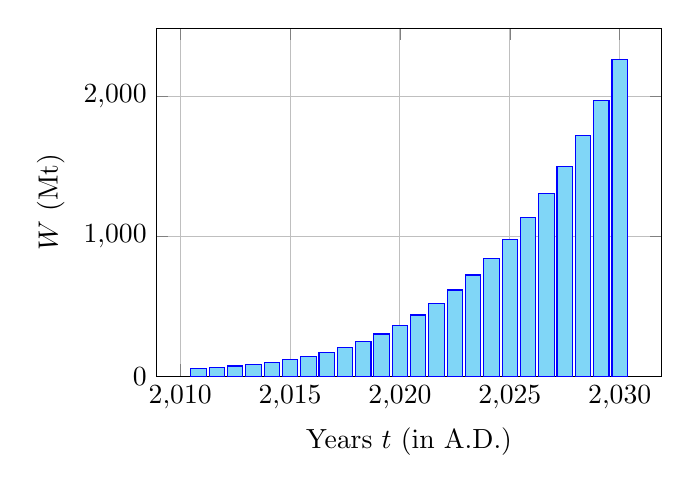
\begin{tikzpicture}
	\begin{axis}[
		width=8cm, height=6cm,
		ymin=0,
		grid=major,
		legend pos=north west,
		xlabel={Years $t$ (in A.D.)},
		ylabel={$W$ (Mt)},
	]
		\addplot[ybar, ybar legend, bar width=0.7, blue, fill=cyan!50, domain=2010:2030] {(4.7531e-164 * exp(0.1887 * x) + 7.7387e281 * exp(-0.3268 * x) * pow(x - 2010.6384, 6.561)) * 1.8};
	\end{axis}
\end{tikzpicture}
\quad
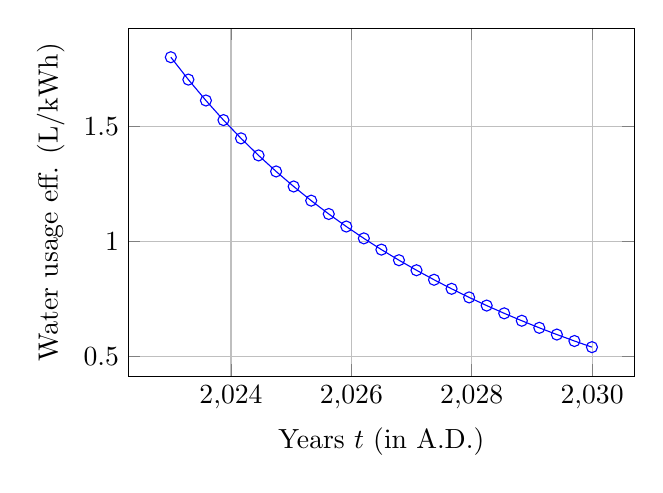
\begin{tikzpicture}
	\begin{axis}[
		width=8cm, height=6cm,
		grid=major,
		legend pos=north west,
		xlabel={Years $t$ (in A.D.)},
		ylabel={Water usage eff. (L/kWh)},
	]
		\addplot[blue, mark=o, domain=2023:2030] {1.8 * 377.5 / (4.7531e-164 * exp(0.1887 * x) + 7.7387e281 * exp(-0.3268 * x) * pow(x - 2010.6384, 6.561))};
	\end{axis}
\end{tikzpicture}
\end{document}